\documentclass[tikz, border=4pt]{standalone}
\usepackage{amsmath}
\usetikzlibrary{arrows.meta, decorations.markings}

% Computational domain and boundary conditions of forBeginners/cavity2d.
% Render the SVG used by the user guide next to this file with
%   pdflatex cavity2dDomain.tex && pdf2svg cavity2dDomain.pdf cavity2dDomain.svg

\begin{document}
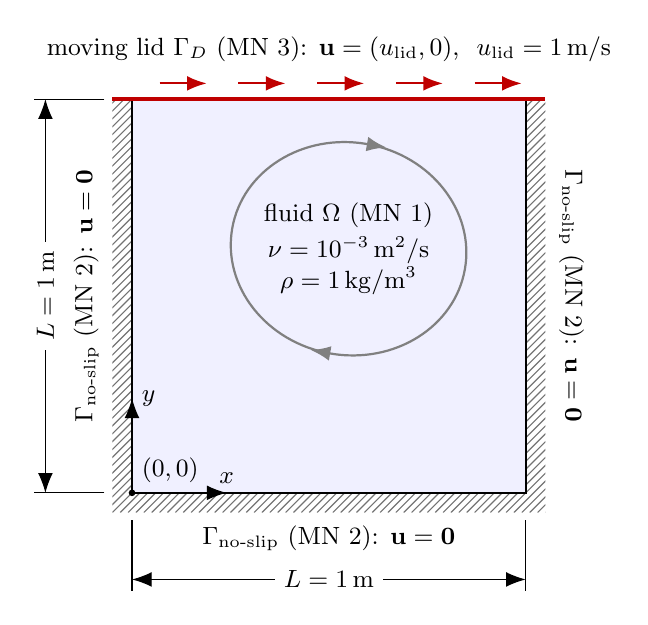
\begin{tikzpicture}[
    >={Latex[length=2.5mm]},
    dim/.style={<->, thin},
    label/.style={font=\small, align=center},
  ]
  \def\L{5}      % side length of the cavity
  \def\w{0.25}   % thickness of the hatched walls

  % fluid domain
  \fill[blue!6] (0,0) rectangle (\L,\L);

  % no-slip walls: left, right and bottom, hatched
  \begin{scope}
    \clip (-\w,\L) -- (-\w,-\w) -- (\L+\w,-\w) -- (\L+\w,\L) -- (\L,\L)
          -- (\L,0) -- (0,0) -- (0,\L) -- cycle;
    \foreach \s in {-5.6,-5.5,...,5.6}
      \draw[black!55, thin] (\s-\w,-\w) -- ++(\L+2*\w,\L+2*\w);
  \end{scope}
  \draw[thick] (0,\L) -- (0,0) -- (\L,0) -- (\L,\L);

  % moving lid
  \draw[very thick, red!75!black] (-\w,\L) -- (\L+\w,\L);
  \foreach \x in {0.35,1.35,...,4.35}
    \draw[->, thick, red!75!black] (\x,\L+0.2) -- (\x+0.6,\L+0.2);

  % sketch of the primary vortex, driven clockwise by the lid
  \draw[gray, thick, postaction={decorate}, decoration={markings,
          mark=at position 0.25 with {\arrow{<}},
          mark=at position 0.75 with {\arrow{<}}}]
    (0.55*\L,0.62*\L) ellipse[x radius=0.3*\L, y radius=0.27*\L, rotate=-10];

  % boundary conditions
  \node[label, above] at (0.5*\L,\L+0.35)
    {moving lid $\Gamma_D$ (MN 3): $\mathbf{u} = (u_\text{lid}, 0)$, \ $u_\text{lid} = 1\,\mathrm{m/s}$};
  \node[label, below] at (0.5*\L,-\w-0.05)
    {$\Gamma_{\mathrm{no\text{-}slip}}$ (MN 2): $\mathbf{u} = \mathbf{0}$};
  \node[label, rotate=90, above] at (-\w-0.05,0.5*\L)
    {$\Gamma_{\mathrm{no\text{-}slip}}$ (MN 2): $\mathbf{u} = \mathbf{0}$};
  \node[label, rotate=-90, above] at (\L+\w+0.05,0.5*\L)
    {$\Gamma_{\mathrm{no\text{-}slip}}$ (MN 2): $\mathbf{u} = \mathbf{0}$};

  % fluid
  \node[label] at (0.55*\L,0.62*\L)
    {fluid $\Omega$ (MN 1)\\[2pt] $\nu = 10^{-3}\,\mathrm{m^2/s}$\\ $\rho = 1\,\mathrm{kg/m^3}$};

  % dimensions
  \draw[dim] (0,-\w-0.85) -- node[fill=white, font=\small] {$L = 1\,\mathrm{m}$} (\L,-\w-0.85);
  \draw[thin] (0,-\w-0.1) -- (0,-\w-1.0) (\L,-\w-0.1) -- (\L,-\w-1.0);
  \draw[dim] (-\w-0.85,0) -- node[fill=white, font=\small, rotate=90] {$L = 1\,\mathrm{m}$} (-\w-0.85,\L);
  \draw[thin] (-\w-0.1,0) -- (-\w-1.0,0) (-\w-0.1,\L) -- (-\w-1.0,\L);

  % coordinate system at the origin of the domain
  \draw[->] (0,0) -- (1.2,0) node[above, font=\small] {$x$};
  \draw[->] (0,0) -- (0,1.2) node[right, font=\small] {$y$};
  \fill (0,0) circle (1.2pt);
  \node[font=\small, above right] at (0,0) {$(0,0)$};
\end{tikzpicture}
\end{document}
